\documentclass[a4paper, 12pt]{article}

% Fontes vectoriais
\usepackage[T1]{fontenc}
\usepackage{ae,aecompl}

% Codificacao dos caracteres
%\usepackage[utf8x]{inputenc}

% Lingua
\usepackage[english]{babel}

% Permitir inclusão de imagens
\usepackage{graphicx}
\usepackage{float}
\usepackage{subfig}

% codigo e comments
\usepackage{verbatim}

% Cores
\usepackage{xcolor}

% Links clicaveis no pdf - Devem ser as ultimas packages a declarar
\usepackage{url}
\usepackage[
bookmarks=true, 
unicode=true,
pdfborder={0 0 0},  
pdftoolbar=true,  
pdfmenubar=true, 
pdffitwindow=true, 
pdftitle={DSLTrans Manual},  
pdfauthor={Claudio Gomes}, 
pdfsubject={DSLTrans},
pdfcreator={LaTeX},
pdfproducer={Texlipse}, 
pdfkeywords={language} {transformation} {dsltrans} {manual},
pdfnewwindow=true,
colorlinks=false,
linkcolor=cyan
]{hyperref}

\newcommand{\HRule}{\rule{\linewidth}{0.5mm}}

\newcommand{\superscript}[1]{\ensuremath{^{\textrm{#1}}}}
\newcommand{\subscript}[1]{\ensuremath{_{\textrm{#1}}}}

\newcommand{\superth}[0]{\superscript{th}}
\newcommand{\superst}[0]{\superscript{st}}
\newcommand{\supernd}[0]{\superscript{nd}}
\newcommand{\superrd}[0]{\superscript{rd}}


\newcommand{\paragraphsize}{8cm}


\begin{document}

\begin{titlepage}

\begin{center}

% Upper part of the page
\includegraphics{imgs/logo.png}\\[1cm]    

\textsc{\LARGE Faculdade de Ci\^{e}ncias e Tecnologia}\\[1.5cm]
\textsc{\LARGE Universidade Nova de Lisboa}\\[1.5cm]

\textsc{\Large Manual}\\[0.5cm]


% Title
\HRule \\[0.4cm]%
{ \huge \bfseries DSLTrans}\\[0.4cm]

\HRule \\[1.5cm]%

% Author and supervisor
\begin{minipage}{0.4\textwidth}
\begin{flushleft} \large
\emph{Authors:}\\
Cl\'{a}udio \textsc{Gomes}\\
Bruno \textsc{Barroca}
\end{flushleft}
\end{minipage}
\begin{minipage}{0.4\textwidth}
\begin{flushright} \large
\emph{Supervisor:} \\
Prof. Dr. Vasco \textsc{Amaral}
\end{flushright}
\end{minipage}

\vfill

% Bottom of the page
{\large \today}

\end{center}

\end{titlepage}


\cleardoublepage

\tableofcontents

\title{DSLTrans: Manual}

\author{Cláudio Gomes$^{\ast}$ \and Bruno Barroca$^{\ast}$ \and Vasco
Amaral$^{\ast}$}

\cleardoublepage

\section*{Versions}

% Deve conter informacoes de versao do documento, com as datas, etc...

\begin{description}
\item[18\supernd August 2011] Initial version.
\end{description}
 
\cleardoublepage

\section{Introduction}
\label{sec:intro}
% Falar de metamodelacao muito por alto em Ecore e
% referencias para mais informacao sobre esta linguagem

Model transformation is the process of converting one or more input models to
one or more output models \cite{model_transformations} where each model
conforms to a metamodel (a set of well formedness rules that specify the abstract
syntax of models and the interrelationships between model elements, i. e., the
set of all possible conformant models \cite{unification_models}) specified using
a metamodeling language that in this case is \emph{Ecore}.

\emph{Ecore} is a subset of the \emph{Unified Modelling Language} (\emph{UML})
and the main language for the creation of metamodels in the \emph{Eclipse
Modelling Framework} (\emph{EMF}) \cite{emf_book}.

\emph{EMF} provides a modelling framework and code generation facility that lets us
define models, from which then we can generate other models or code for building
tools and other applications \cite{emf_book} \footnote{For more
information about the \emph{Ecore} language and \emph{EMF} refer to
\url{http://www.eclipse.org/modeling/emf/?project=emf}}.

Figure \ref{fig:model_trans_general} shows the model transformation process. We
can see that every model involved has to conform to some metamodel. At the
highest level, the metametamodel conforms to itself meaning that its structure
can be expressed with the same terms it describes. The rules that make
up the transformation process are also expressed in a model that is interpreted
by some engine that takes some input models and generates some output
models.

\begin{figure}[h]
\begin{center}
  \includegraphics[scale=0.6, trim=3.3cm 13.6cm 3.1cm 0.7cm,
  clip]{imgs/model_transformation.pdf}
  \caption{Model transformation process and required elements.}
  \label{fig:model_trans_general}
\end{center}
\end{figure}

\clearpage

\subsection{What is \emph{DSLTrans}?}

\emph{DSLTrans} is a language specifically designed to support the definition of
\emph{Ecore}-based model transformations \cite{dsltranslator}. It is particularly
useful when building a new language (for instance, a language to describe graphical
user interfaces) whose semantics are not known and it is necessary
to express them in terms of an existing well known language (a Java
application\footnote{Java code can be modelled using an \emph{Ecore}-based metamodel
thus making it possible to treat Java applications as models}).

The process of assigning meaning to a new language trough transformations
involves coming up with a set of mappings between the terms of the source
language to terms in the target language \cite{dsltranslator}. In \emph{DSLTrans} those
mappings are expressed in the form of rules where the first part of each rule
has a pattern describing some arrangement of terms in the source language and
the second part has the terms to be created in case the first part exists in
some input model.

Figure \ref{fig:model_trans_manual} shows the model transformation process
according to the technologies and tools used throughout this manual. As you can
see, \emph{DSLTrans} is a metamodel used to express transformations that are
interpreted by the \emph{DSLTranslator} engine to translate models.


\begin{figure}[h]
\begin{center}
  \includegraphics[scale=0.6, trim=3.3cm 13.6cm 3.1cm 0.7cm,
  clip]{imgs/model_transformation_dsltrans.pdf}
  \caption{Model transformation process and required elements used throughout
  this manual.}
  \label{fig:model_trans_manual}
\end{center}
\end{figure}

\clearpage

\subsubsection{A Metaphor}
\label{subsubsec:metaphor}
% Da um exemplo de transformacao, realcando a questao dos mapping 1-1. Tem
% informacao desta no manual do dsltrans.

In order to better understand all these concepts, lets focus on a simple example where
we have a small language (a.k.a. a metamodel) used to define an individual's genealogy tree and we will come up with transformations that present information from some genealogy tree (a.k.a. model) in different views.

Figure \ref{fig:genealogy_tree_example} shows an example of a genealogy tree. We
can see that John and Mary married and had one son: Thomas who in turn married
Sarah\ldots and so on.

\begin{figure}[h]
\begin{center}
  \includegraphics[scale=1, trim=4.1cm 17.4cm 4.1cm 3.6cm,
  clip]{imgs/genealogy_tree_example.pdf}
  \caption{Genealogy tree example.}
  \label{fig:genealogy_tree_example}
\end{center}
\end{figure}

How can we find out, given a tree of any size, who are the couples? More
specifically we want as a result of the transformation a set of couples like the
one shown in figure \ref{fig:couples_example}.

\begin{figure}[h]
\begin{center}
  
\includegraphics[scale=1, trim=5.6cm 21.0cm 8.4cm 3.8cm,
  clip]{imgs/couples_example.pdf}
  \caption{Couples set example.}
  \label{fig:couples_example}
\end{center}
\end{figure}

The transformation rules have to be based on patterns as described earlier so
something like figure \ref{fig:gen_to_couple_example} should be fine. The
transformation is only made of a single rule, that says the following:
\emph{Every person that is married to other person in the source model becomes
the same person associated with the same other person in the target (or output) model.}
Notice that the connections in the source model are different
than those in the target model.

\begin{figure}[h]
\begin{center}
  \includegraphics[scale=0.9, trim=3.5cm 21.5cm 3.8cm 4.2cm,
  clip]{imgs/gen_to_couple_example.pdf}
  \caption{Genealogy to Couples transformation.}
  \label{fig:gen_to_couple_example}
\end{center}
\end{figure}


Another way of looking at the transformation is by defining two rules: one
establishing the fact that \emph{every married couple in the source metamodel becomes two
individuals in the target} and afterwards \emph{add} the relation between those
two individuals, forming a couple. Figure \ref{fig:gen_to_couple_example_extended} illustrates this approach. Notice that the dashed links between the source and
target model elements mean that in the bottom rule we don't want to create new
elements in the target model: we only want to create a connection between them.

Although partitioning the transformation and referring
to elements that already exist in the output model\footnote{because these elements where generated by some previous rule} may seem too much work and counter-intuitive; for complex transformations it is a more natural way since we start by looking only to each
element individually and expressing its meaning in the target language through simple rules, then we explore more and more complex patterns saying what those
mean.


\begin{figure}[h]
\begin{center}
  \includegraphics[scale=0.9, trim=3.5cm 17.0cm 3.8cm 4.2cm,
  clip]{imgs/gen_to_couple_example_extended.pdf}
  \caption{Genealogy to Couples transformation - Partitioned.}
  \label{fig:gen_to_couple_example_extended}
\end{center}
\end{figure}


\clearpage

\subsection{DSLTrans and Other Transformation Languages}
\label{subsubsec:other_languages}

There are several papers about transformation languages. Bellow is a brief description of some of them so you can have an idea about their general features with respect to \emph{DSLTrans}.


\subsubsection{QVT} 

Query / View / Transformation is a standard defined by the
\emph{Object Management Group}; its implementation is \emph{SmartQVT}: a
tool that compiles model transformations specified in QVT to produce Java code
used to perform these transformations \cite{qvt_transformation_language}.

\subsubsection{ATL} 

\emph{Atlas Transformation Language} is a transformation
language inspired by the \emph{QVT} requisites that uses the \emph{OCL}
formalism. It provides declarative constructs as we used in the previous example
and, for the most difficult transformations, it allows the user to define
imperative rules, which increases its flexibility and complexity
\cite{atl_transformation_tool}.

\subsubsection{ATC} 

\emph{Atomic Transformation Code} is a low level model transformation language
with the main purpose of being the target for other transformation
languages' specifications allowing for the execution of a diversity of model
transformation languages via translation to \emph{ATC} \cite{atc_user_guide}.


\subsubsection{ETC}

\emph{Epsilon Transformation Language} is an hybrid\footnote{ An hybrid transformation language is one that provides both imperative and
declarative constructs, as \emph{ATL}, \emph{ETC}, and others.}, rule-based model-to-model transformation language that has the flexibility of allowing for query, navigation and
modification of multiple target and source models \cite{epsilon_eclipse}.


\subsubsection{MOLA}

\emph{MOdel transformation LAnguage}, similarly to \emph{DSLTrans}, is a graphical
transformation language that strives to produce readable transformations by
combining traditional structured programming in a graphical form with simple
pattern rules \cite{mola_trans_language}.


\subsubsection{RubyTL}

\emph{Ruby Transformation Language} is a domain specific hybrid
transformation language embedded in Ruby that provides an extension
mechanism based on plugins \cite{rubytl}.

\subsubsection{UMLX}

\emph{UMLX} is a graphical transformation language that extends \emph{UML}
through the use of transformation diagrams that are no more than class diagrams
with additional relations to specify mappings between input and
output models \cite{umlx}.

\subsubsection{GReAT}

The Graph REwriting And Transformation is a rule-based graphical language that,
as DSLTrans, sees models as labelled graphs and uses graph
transformation formalisms to translate them \cite{great}.

\subsubsection{\textbf{DSLTrans}}

With respect to the described transformation languages, \emph{DSLTrans} is a
rule-based graphical transformation language\footnote{The latest version of DSLTrans supports also textual syntax for transformation specification} that uses declarative constructs and graph formalisms to prescribe transformations. A distinctive characteristic is that all the
transformations specified in \emph{DSLTrans} are guaranteed to terminate\footnote{DSLTrans
transformations are guaranteed to terminate because the language doesn't
support loop constructs and no rule can be applied forever. This means the
language is not Turing complete but there are techniques that allows us to
build complex and still readable transformations as you will see.}.
This means the language is not Turing complete and for very complex transformations it might not be the ideal transformation language.
% TODO Colocar aqui definicao de traducao e transformacao se o bruno responder ao email.



% TODO A brief history of DSLtrans
% \subsection{\emph{DSLTrans} Biography}


\clearpage

\subsection{Assumptions}

\subsubsection{User}

% Descreve as assuncoes que fazemos acerca do utilizador:
% - Sabe metamodelar . . . etc
About the reader of this manual and hopefully user of \emph{DSLTrans} we make
the following assumptions:

\begin{description}
  \item[Modelling Jargon] The reader should be familiar with the modelling terms
  like model, metamodel, metametamodel, model transformation, language,
  etc\ldots. \cite{unification_models} and \cite{model_transformations} give
  readable overviews of most of the terms used throughout this manual.
  \item[Eclipse Modelling Framework and Ecore] The user knows how to use the EMF
  main metamodeling language to created metamodels and respective instances. For
  more information refer to the project's home
  (\url{http://www.eclipse.org/modeling/emf/}) or read the EMF book in
  \cite{emf_book}. There is also a good tutorial on how to create
  metamodels here:
  \url{http://tinyurl.com/3oo8woz} 
  \item[Advanced System User] We assume that the user knows how to change
  environment variables and install software in its system.
\end{description}


\subsubsection{Environment}

% Descrever as caracteristicas exactas do software usado.
% - Deve ter uma indicacao precisa do sofware usado, nomeadamente, versao de
% eclipse e versao dos plugins do dsltrans.
In order to succeed in learning DSLTrans and following the examples presented in
this manual it is highly recommended that you have the following tools:

\begin{itemize}
  \item Eclipse Modeling Tools, Helios Service Release 2. You should be able to
  download it in the eclipse home page \url{http://www.eclipse.org}. After
  starting eclipse and going to \emph{Help, About Eclipse}, you should see the
  version info shown in figure \ref{fig:rec_eclipse_version}.
  \item SWI-Prolog version 5.10.4 by Jan Wielemaker. The \emph{DSLTranslator}
  engine uses the Prolog language internally to process the transformations. You should
  be able to download SWIProlog from the project's home page
  \url{http://www.swi-prolog.org/}. Figure \ref{fig:rec_prolog_version} shows
  Prolog's version info.
\end{itemize}


\begin{figure}[H]
\begin{center}
  \includegraphics[width=0.9\textwidth]{imgs/eclipse_version.jpg}
  \caption{Recomended eclipse version.}
  \label{fig:rec_eclipse_version}
\end{center}
\end{figure}

\begin{figure}[H]
\begin{center}
  \includegraphics[width=0.9\textwidth]{imgs/prolog_version.jpg}
  \caption{Recomended prolog version.}
  \label{fig:rec_prolog_version}
\end{center}
\end{figure}


\begin{comment} 

Eclipse:
	Eclipse version: Eclipse Modeling Tools Helios Release
	
	Plugins:
		dsltransAnalysis_1.0.0.201107201833.jar
		DSLTransEditor.diagram_1.0.0.201008111406.jar
		DSLTransEditor.editor_1.0.0.jar
		DSLTransEditor.edit_1.0.0.jar
		DSLTransEditor_1.0.0.jar
		DSLTranslator_1.0.2.jar
		mprolog_1.0.0.201107201759.jar
		text_1.0.0.jar
		Transformer2.0_1.0.2.jar

WINDOWS:
	SWI Prolog version 5.10.x
	
		
LINUX:

			

\end{comment}

\clearpage

\subsection{About this Manual}


\subsubsection{Objectives}

After reading this manual the user should be able to:

\begin{itemize}
  \item Create and read \emph{DSLTrans} transformations either from scratch or by using
  prototyping techniques.
  \item Understand how higher order transformations work and even
  better: create them.
  \item Understand the advantages and limitations of \emph{DSLTrans} and
  when to use it instead of other transformation languages like ATL
  \cite{atl_transformation_tool}, \emph{SmartQVT}
  \cite{qvt_transformation_language} or others presented in page
  \pageref{subsubsec:other_languages}.
\end{itemize}


%\subsubsection{Notations}

% TODO Falar um pouco sobre as notacoes usadas no manual, estrutura, etc \ldots

\subsubsection{Structure}

% TODO O leitor deve ler com atencao a seccao de quickstart pois eh altamente
% recomendada e ensina muito!
If you are new to \emph{DSLTrans}, you should read
this manual from the beginning to at least section \ref{sec:language_def}. The
first sections are the ones that will help you understand the main concepts
behind the \emph{DSLTrans} and the remaining can be used as a reference.

This manual is divided in five sections:

\begin{description}
  \item[Installation] Where you will learn how to get the needed
  tools up and running so that you can follow the rest of this manual's examples
  and tutorials.
  \item[Quick Start] This section presents a hands on approach to
  \emph{DSLTrans} with a tutorial on how to create the transformation described
  in section \ref{subsubsec:metaphor} in two different ways. While it teaches
  you how to use \emph{DSLTrans}, it explains the main concepts and procedures
  involved in the creation of a transformation.
  \item[Language Definition] Where each element of a transformation is described
  and some examples in both graphical and textual syntax are given to help you
  understand how it can be used; possible restrictions and good practices are
  present. This section can be used as a reference as it contains the
  description of every element in the language.
  \item[Advanced Topics] Once you know how to use \emph{DSLTrans} well enough
  you will want to avoid some repetitive tasks when building most of the
  transformations. Since \emph{DSLTrans} is a metamodeled language it is
  possible to use it to transform transformations. This section focusses in
  teaching you how to use (and build) higher order transformations and to build
  complex transformation to simulate the stepping of abstract machines and even
  how to create transformations that are specific to some domain.
  \item[FAQ] Frequently asked questions and common errors are
  answered here.
\end{description}

\clearpage

\cleardoublepage

\section{Installation}

\subsection{Windows7 \& Vista}

In order to successfully follow the examples in this manual and use
\emph{DSLTrans} you have to follow (carefully) these steps:

Download and install SWI-Prolog version 5.10.4.

Download and extract Eclipse Modeling Tools, Helios Service Release 2.

Set the environment variables shown in the figures \ref{fig:path_user}
and \ref{fig:path_system} below.

\begin{figure}[h]
\begin{center}
  \includegraphics[scale=0.9]{imgs/path_user.jpg}
  \caption{Path to add to the \emph{user} \emph{Path} variable.}
  \label{fig:path_user}
\end{center}
\end{figure}

Note that you have to replace \verb=C:\Program Files\Java\jdk1.6.0_26\bin=
for your system's Java bin directory. Also, beware that the environment
variable you have to edit is the \emph{user} Path variable.

\begin{figure}[h]
\begin{center}
  \includegraphics[scale=0.9]{imgs/path_system.jpg}
  \caption{Path to add to the \emph{system} \emph{Path} variable.}
  \label{fig:path_system}
\end{center}
\end{figure}

You have to replace \verb=C:\Program Files\pl\bin= for your prolog installation
bin directory too. This time the variable to edit is the \emph{System} Path
variable.

Now you have to copy the \verb=jpl.jar= file, in the 
\verb=C:\Program Files\pl\lib= 
directory, and paste it in Java's lib directory: 
\verb=C:\Program Files\Java\jdk1.6.0_26\lib=.

\begin{figure}[h]
\begin{center}
  \includegraphics[width=0.8\textwidth]{imgs/jpl_cpy.jpg}
  \caption{Prolog's jpl.jar copied to Java's lib directory.}
  \label{fig:jpl_cpy}
\end{center}
\end{figure}

Finally, you need to install the DSLTrans plugins, placing them in the
eclipse plugins directory (e.g., \verb=C:\Users\clagms\Desktop\eclipse\plugins=)


\begin{figure}[h]
\begin{center}
  \includegraphics[width=\textwidth]{imgs/dsltrans_plugins_cpy.jpg}
  \caption{DSLTrans plugins being copied to eclipse's plugins directory.}
  \label{fig:dsltrans_plugins_cpy}
\end{center}
\end{figure}

\clearpage


\begin{comment}	

Download & Install Prolog

Download & Install Plugins

Handle java library path

Path do admin com C:\Program Files\pl\bin

Copy jpl.jar to lib java folder

\end{comment}



% \subsection{Linux}
% TODO

\cleardoublepage

\section{Quick Start}
\label{sec:quick_start}

% Esta seccao deve ter um pequeno tutorial a demonstrar como fazer uma
% transformacao muito simples.

% Colocar transformacao de GenealogyTree pra algum target bom.

In this section you will create the two transformations
described in page \pageref{subsubsec:metaphor} using \emph{DSLTrans} graphical
syntax.

\subsection{Metamodels}

First step is to build the required metamodels: \emph{GenealogyTree} and
\emph{Couples}. Both were built using \emph{Ecore Diagram Editor} and are shown
in figures \ref{fig:genealogy_tree_mm} and \ref{fig:couples_mm}. 

\begin{figure}[h]
\begin{center}
  \subfloat[GenealogyTree.]{\label{fig:genealogy_tree_mm}\includegraphics[width=0.45\textwidth]{imgs/GenealogyTree.pdf}}
  \subfloat[Couples.]{\label{fig:couples_mm}\includegraphics[width=0.45\textwidth]{imgs/Couples.pdf}}
  \caption{Metamodels.}
  \label{fig:genTree_couples_metamodels}
\end{center}
\end{figure}

Notice that in the \emph{Couples} metamodel the notion of parenting
relationship between \emph{Couples} is kept. For a given couple to be
directly connected to other couple it means that the first one gave birth to one
of the elements of the second couple.

\clearpage

\subsection{Example Model}
\label{subsec:creating_example_model}

To test the transformation you will need an example model. Open the
\emph{GenealogyTree.ecore} file and click on \emph{Create Dynamic
Instance\ldots}. Name the new file as \emph{GenealogyTree.xmi} (see figure
\ref{fig:create_dinamic_instance} ). It is important that you name it like that
to avoid confusion later in this tutorial.


\begin{figure}[h]
\begin{center}
  \includegraphics[scale=0.7]{imgs/create_dinamic_instance.jpg}
  \caption{Dynamic Instance Creation.}
  \label{fig:create_dinamic_instance}
\end{center}
\end{figure}

Then open the created file (\emph{GenealogyTree.xmi}) and create a model based
on figure \ref{fig:genealogy_tree_example} in page
\pageref{fig:genealogy_tree_example}. Your model should look like the one shown
in figure \ref{fig:genealogical_tree_example_model}. Don't forget to fill the
\emph{Children}, \emph{Husband} and \emph{Wife} properties (in eclipse's
properties view) for each \emph{Marriage}, where appropriate.

\begin{figure}[h]
\begin{center}
  \includegraphics[scale=0.7]{imgs/genealogical_tree_example_model.jpg}
  \caption{\emph{GenealogyTree} Example Model.}
  \label{fig:genealogical_tree_example_model}
\end{center}
\end{figure}

\clearpage

\subsection{Planning the Transformation}

In page \pageref{subsubsec:metaphor} we had two ways of expressing the
transformation to generate \emph{Couples} models: a simple one and an extended,
more partitioned, version.

Informally, if we ignore the parenting relationship between couples, we can say
that a couple is a \emph{Couple} element, together with
the respective \emph{husband} and \emph{wife} \emph{Persons}. So we only have to
match the
\emph{Persons} and \emph{Marriage} elements in the \emph{GenealogyTree}
metamodel.

It is advised that before you start building the transformation, you write down
the basic rules (or steps if you prefer) that make it up. For this case study
ignore the parenting relationship between \emph{Couples} and use the following
rules:

\begin{enumerate}
  \item Every \emph{Marriage}, \emph{husband} and \emph{wife} \emph{Persons} in
  the \emph{GenealogyTree} becomes a \emph{Couple}, \emph{husband} and
  \emph{wife} \emph{Persons} in the \emph{Couples} model;
  \item Every \emph{Couple} generated has to be connected with the
  \emph{CouplesSet} (root) element.
\end{enumerate}

\clearpage

\subsection{Understanding DSLTrans Overall Semantics}

A \emph{DSLTrans} transformation is composed of multiple
\emph{layers}, each with several \emph{rules}. A \emph{rule} has a match side -
where a pattern is matched against some input model - and an apply side - where a pattern is
created in the output model. It is applied while there are elements
in the input model that satisfy the match pattern. In a \emph{layer}, all the
\emph{rules} are executed in a non-deterministic fashion while \emph{layers} are
executed sequentially following the \emph{previous source} association.

\clearpage

\subsection{Creating a Blank Transformation}

Now that you have an idea of the rules needed and how a transformation is
processed, you can start creating a blank transformation.

First open the \emph{New File Wizard} and select \emph{DSLtrans Diagram} inside
the \emph{Examples} category (see figure \ref{fig:create_dsltransformation_1}).

\begin{figure}[h]
\begin{center}
  \includegraphics[scale=0.6]{imgs/create_dsltransformation_1.jpg}
  \caption{New File Wizard.}
  \label{fig:create_dsltransformation_1}
\end{center}
\end{figure}

\emph{DSLTrans} transformations are nothing but models conforming to the
\emph{DSLTrans} metamodel. According to \emph{EMF}, the abstract
definition of models is expressed in the \emph{XML Metadata
Interchange} (\emph{XMI}) \cite{xmi_omg}. Since you are using the graphical
syntax to build the transformation, the new \emph{DSLtrans Diagram} wizard will create two files:
\begin{description}
  \item[NewTransformation.dsltrans]	This file contains the transformation model
  in \emph{XMI} format. See figure \ref{fig:create_dsltransformation_3}.
  \item[NewTransformation.dsltrans\_diagram] This file contains the additional
  information needed to create and position the transformation elements in a
  diagram. See figure \ref{fig:create_dsltransformation_2}.
\end{description}

\begin{figure}[h]
\begin{center}
  \includegraphics[scale=0.6]{imgs/create_dsltransformation_3.jpg}
  \caption{Setting model name.}
  \label{fig:create_dsltransformation_3}
\end{center}
\end{figure}

\begin{figure}[h]
\begin{center}
  \includegraphics[scale=0.6]{imgs/create_dsltransformation_2.jpg}
  \caption{Setting diagram name.}
  \label{fig:create_dsltransformation_2}
\end{center}
\end{figure}

\clearpage

\subsection{DSLtrans Diagram Editor}

After creating and opening a new \emph{DSLTrans} file, you will see a window
like the one shown in figure \ref{fig:dsltrans_editor_window}.

While building a transformation you will frequently use:
\begin{itemize}
  \item The \emph{Properties} window to set package names and other properties
  of the transformation elements;
  \item The \emph{Palette} is used to add new elements to the transformation
  (e.g., \emph{rules}, match classes, etc\ldots) and connections among them;
  \item The \emph{Outline} view to get an idea of the overall structure of the
  transformation and navigate easily trough complex diagrams;
\end{itemize}

\begin{figure}[h]
\begin{center}
  \includegraphics[width=\textwidth]{imgs/dsltrans_editor_window.jpg}
  \caption{DSLTrans Diagram Editor Window.}
  \label{fig:dsltrans_editor_window}
\end{center}
\end{figure}

\clearpage

\subsection{Defining the Transformation}

A transformation can have multiple input and output models but for this example
you only need one input and one output. To set the input for the transformation
you will add a new \emph{FilePort} by clicking it in the objects section of the
\emph{Palette} and clicking again in the diagram. After this you should see
something like figure \ref{fig:file_port_add}.


\begin{figure}[h]
\begin{center}
  \subfloat[FilePort
  Palette.]{\label{fig:click_file_port}\includegraphics[width=0.3\textwidth]{imgs/click_file_port.jpg}}
  \subfloat[FilePort
  Diagram.]{\label{fig:after_click_file_port}\includegraphics[width=0.3\textwidth]{imgs/after_click_file_port.jpg}}
  \caption{Adding a new element - FilePort.}
  \label{fig:file_port_add}
\end{center}
\end{figure}

Then you should set the \emph{FilePort}'s properties in the \emph{Properties}
window as in figure \ref{fig:file_port_properties}. Notice that the
\emph{Name} property can be anything. Just write something meaningful for the
sake of readability.

\begin{figure}[h]
\begin{center}
  \includegraphics[scale=0.7]{imgs/file_port_properties.jpg}
  \caption{FilePort properties.}
  \label{fig:file_port_properties}
\end{center}
\end{figure}

For every input model of a \emph{DSLTrans} transformation, the metamodel it
conforms to must be stated. To do that, you add a \emph{MetaModelIdentifier}
inside the \emph{FilePort} previously created. Then set the properties as in
figure \ref{fig:meta_id_properties}.

\begin{figure}[h]
\begin{center}
  \includegraphics[scale=0.7]{imgs/meta_id_properties.jpg}
  \caption{MetaModelIdentifier properties.}
  \label{fig:meta_id_properties}
\end{center}
\end{figure}

Beware that \emph{Meta Model Name} as to be always in the format
\verb=package.Package=. The \verb=package= value is the metamodel root package
(see figure \ref{fig:package_name}). By default, this is the name of the
metamodel in lower case letters.


\begin{figure}[h]
\begin{center}
  \includegraphics[scale=0.7]{imgs/package_name.jpg}
  \caption{GenealogyTree metamodel package name.}
  \label{fig:package_name}
\end{center}
\end{figure}


Now that the input is well known and identified, you can proceed to add a
first \emph{Layer} by the same procedure as described earlier to add elements to the
transformation. As for its properties it is only recommended that
you set the \emph{Name} and \emph{Description} to something meaningful.

The next step is to connect the input \emph{FilePort} to the first \emph{Layer}
using a \emph{PreviousSource} association. To add this connection you have to
first click in the \emph{PreviousSource} in the \emph{Palette}, then click in
the \emph{Layer} and drag the connection to the \emph{FilePort}. The result is
in figure \ref{fig:after_previous_source}. Don't be misled by the fact that the
arrows points downwards while you dragged it upwards. It
shows the flow of the information but its name is \emph{PreviousSource}.

\begin{figure}[h]
\begin{center}
  \includegraphics[scale=0.7]{imgs/after_previous_source.jpg}
  \caption{Transformation after adding the PreviousSource Association.}
  \label{fig:after_previous_source}
\end{center}
\end{figure}

Each \emph{Layer} has an output. You can set that output to a file (by setting
the \emph{Output File Path URI} property) if you want to see the outcome of the
transformation at a specific \emph{Layer}. This is great for debugging purposes.
You should set the \emph{Output File Path URI} property to \emph{Couples.xmi}.
Even if there is no external output set, the outcome of a
layer is always validated against it's metamodel. Because of it you have to
create a \emph{MetaModelIdentifier} pointing to the output metamodel for each layer.
Figure \ref{fig:metamodelid_l1} shows the properties of this
\emph{MetaModelIdentifier}.


\begin{figure}[h]
\begin{center}
  \includegraphics[scale=0.7]{imgs/metamodelid_l1.jpg}
  \caption{\emph{MetaModelIdentifier} properties.}
  \label{fig:metamodelid_l1}
\end{center}
\end{figure}


As for the rules in this \emph{layer}, we only need one: to create the root
element of the output model. It has to be like this because in the next layers
new elements will be generated and they need to be ``attached'' to the root
element as described in the \emph{Couples} metamodel. Don't worry if you can't
understand everything yet, keep going, you're almost there!

Now insert a \emph{Rule} in the recently created \emph{Layer} and set its
description to something that describes the main purpose of the \emph{Rule}
(e.g., root element). After that, insert a \emph{MatchModel} and an
\emph{ApplyModel} in the top and bottom parts of the \emph{Rule}, respectively
(see figure \ref{fig:root_elements_empty_rule}).

\begin{figure}[h]
\begin{center}
  \includegraphics[scale=0.7]{imgs/root_elements_empty_rule.jpg}
  \caption{Root Elements rule with empty match and apply models.}
  \label{fig:root_elements_empty_rule}
\end{center}
\end{figure}

According to figure \ref{fig:genTree_couples_metamodels} the root element of the
\emph{GenealogyTree} metamodel is the \emph{GenealogyTree} element and the root
of the \emph{Couples} metamodel is the \emph{CouplesSet} element.

The purpose of this rule is to say that for every \emph{GenealogyTree} element
in the input model, you want to generate a \emph{CouplesSet} element in the
output model. Figure \ref{fig:rule_match_apply_class} shows the
\emph{AnyMatchClass} and the \emph{ApplyClass} elements created inside the respective containner models
created previously. As for the properties of each inserted element, set them
according to figure \ref{fig:match_apply_classes_properties}.

\begin{figure}[h]
\begin{center}
  \includegraphics[scale=0.7]{imgs/rule_match_apply_class.jpg}
  \caption{AnyMatchClass and ApplyClass elements.}
  \label{fig:rule_match_apply_class}
\end{center}
\end{figure}

\begin{figure}[h]
\begin{center}
  \subfloat[GenealogyTree
  AnyMatchClass
  properties.]{\label{fig:genealogy_properties_match}\includegraphics[width=0.35\textwidth]{imgs/genealogy_properties_match.jpg}}
  \subfloat[CouplesSet ApplyClass element
  properties.]{\label{fig:couplesset_properties_apply}\includegraphics[width=0.35\textwidth]{imgs/couplesset_properties_apply.jpg}}
  \caption{Match and Apply Pattern properties.}
  \label{fig:match_apply_classes_properties}
\end{center}
\end{figure}

Now would be a good time to test the transformation. The transformation has one
\emph{FilePort} that points to a \emph{GenealogyTree.xmi} file where the input
model is (you created it in section \ref{subsec:creating_example_model}); and
one \emph{Layer} whose output is a file named \emph{Couples.xmi}, where the
output model will be.

To run the transformation, just right-click in
\emph{TransformationName.dsltrans}, \emph{DSLTranslator} and
\emph{Transform}, as in figure \ref{fig:transform_dsltrans}. You should see some
debugging output in the console view. If any error occurs, refer to section
\ref{sec:faq} in page \pageref{sec:faq}.

\begin{figure}[h]
\begin{center}
  \includegraphics[scale=0.7]{imgs/transform_dsltrans.jpg}
  \caption{Executing a transformation.}
  \label{fig:transform_dsltrans}
\end{center}
\end{figure}

If everything went well you should see a new file named \emph{Couples.xmi} on
your project. Open it and you will see that the model only contains the root
element (see figure \ref{fig:couples_xmi_1}). This makes sense since the
transformation only matches \emph{GenealogyTree} elements to produce
\emph{CouplesSet} elements and there is only one \emph{GenealogyTree} element in
the input model.

\begin{figure}[h]
\begin{center}
  \includegraphics[scale=0.7]{imgs/couples_xmi_1.jpg}
  \caption{Couples resulting model.}
  \label{fig:couples_xmi_1}
\end{center}
\end{figure}


It's time to add a second \emph{Layer} to the transformation. Don't forget to
identify the output metamodel using the \emph{MetaModelIdentifier} as
previously. The properties of the \emph{Layer} and \emph{MetaModelIdentifier}
are the same except theres is a new \emph{Previous Source} association between
the second \emph{Layer} and the first one, as figure
\ref{fig:second_layer_empty} illustrates.

\begin{figure}[h]
\begin{center}
  \includegraphics[scale=0.7]{imgs/second_layer_empty.jpg}
  \caption{New \emph{Layer} with \emph{Previous Source} association.}
  \label{fig:second_layer_empty}
\end{center}
\end{figure}

The second \emph{Layer} will have rules that match \emph{Marriages} in order to
generate \emph{Couples}. The skeleton of the \emph{Rule} to add is quite simple
(see figure \ref{fig:second_rule_skeleton}). Beware that you need to add
\emph{Match} and \emph{Apply} models to each side of the \emph{Rule} before
adding the \emph{AnyMatchClasses} and \emph{ApplyClasses}.

\begin{figure}[h]
\begin{center}
  \includegraphics[scale=0.7]{imgs/second_rule_skeleton.jpg}
  \caption{Second Rule Skeleton.}
  \label{fig:second_rule_skeleton}
\end{center}
\end{figure}

On the top of the \emph{Rule} it is necessary to match a \emph{Marriage} and the
two associated \emph{Persons}, so go ahead and set the appropriate properties
for three of the four \emph{AnyMatchClasses} in the \emph{MatchModel} (see
figure \ref{fig:second_rule_skeleton_2}). Since a \emph{Couple} and two
\emph{Persons} will be generated by this \emph{Rule}, set the properties of the
\emph{ApplyCasses} according to figure \ref{fig:second_rule_skeleton_2}. It is
very important that you set the \emph{PackageName} property of each \emph{Rule}
element. In this case we set the \emph{PackageName} of \emph{AnyMatchClasses} to
\verb=genealogytree=  and the \emph{ApplyClasses} with \verb=couples= (as
in the previous \emph{Layer}).

\begin{figure}[h]
\begin{center}
  \includegraphics[scale=0.7]{imgs/second_rule_skeleton_2.jpg}
  \caption{Second Rule with class names.}
  \label{fig:second_rule_skeleton_2}
\end{center}
\end{figure}

The generated elements \emph{Couple} and \emph{Person's} need to be associated
with each other and with the root element \emph{CouplesSet} according to the
\emph{Couples} metamodel. To create associations between apply elements you have
to insert \emph{Apply Associations}, click and drag. Insert the needed
associations between the generated elements according to figure
\ref{fig:couple_relations}. Notice that the direction of the
\emph{ApplyAssociations} and their names correspond to the associations
declared in the metamodel. This is very important since \emph{DSLTrans} will
check the generated model correctness and won't allow models that do not conform to
the metamodel.

\begin{figure}[h]
\begin{center}
  \includegraphics[scale=0.7]{imgs/couple_relations.jpg}
  \caption{Generated \emph{Couple} associations.}
  \label{fig:couple_relations}
\end{center}
\end{figure}

The generated \emph{Couples} need to be related to the root element
\emph{CouplesSet}. Set the properties of the last \emph{ApplyClass} and insert
the association as shown in figure \ref{fig:couple_relations_2}.

\begin{figure}[h]
\begin{center}
  \includegraphics[scale=0.7]{imgs/couple_relations_2.jpg}
  \caption{Generated \emph{Couple} associations with \emph{CouplesSet}.}
  \label{fig:couple_relations_2}
\end{center}
\end{figure}

If you start asking why do we want to generate more \emph{CouplesSet} elements,
then you are in the right track! In this rule you want to add new elements
(\emph{Couple} and \emph{Persons}) but connect them to the previously
generated \emph{CouplesSet} element. How do you say in \emph{DSLTrans} that you
don't want to generate a new \emph{CouplesSet} element but instead want to
use the previously generated one? The answer is to add a
\emph{PositiveBackwardRestriction} between the generated element and one of the
elements that generated it. In this case the generator element is the
\emph{GenealogyTree} and the generated one is the \emph{CouplesSet}. Insert a
\emph{PositiveBackwardRestriction} between the \emph{GenealogyTree} and the
\emph{CouplesSet} and set the required properties so that the \emph{Rule} looks
like the one in figure \ref{fig:rule_without_match_pattern}. Don't forget to set
the appropriate \emph{Package Names}, it's one of the most common errors (see
section \ref{sec:faq}).

\begin{figure}[h]
\begin{center}
  \includegraphics[scale=0.7]{imgs/rule_without_match_pattern.jpg}
  \caption{Rule with a \emph{PositiveBackwardRestriction}.}
  \label{fig:rule_without_match_pattern}
\end{center}
\end{figure}

The apply pattern of the \emph{Rule} is complete and the match elements only
need associations between them. To express that the two
\emph{Person's} are in the same \emph{Marriage}, you have
\emph{PositiveMatchAssociations}. They work much in the same way as the
\emph{ApplyAssociations} in the apply pattern, except they are inserted among
match elements. Insert the required associations so that your match pattern
looks like the one in figure \ref{fig:match_pattern_marriages}.

\begin{figure}[h]
\begin{center}
  \includegraphics[scale=0.7]{imgs/match_pattern_marriages.jpg}
  \caption{Match pattern with \emph{PositiveMatchAssociations}.}
  \label{fig:match_pattern_marriages}
\end{center}
\end{figure}

Now the rule (and the transformation) is almost complete. However, an important
detail is missing and without it the transformation won't work: when using
\emph{PositiveBackwardRestrictions} you are matching previously generated and
generator elements. \emph{DSLTranslator} internally keeps track of these elements but
only if you say so, or else executing a large transformation would consume a
lot of memory. In order to tell \emph{DSLTranslator} to save traceability links between
generated and generator elements you have to place an \emph{ApplyAttribute}
in the generated elements in the moment they are first created and then use the
same \emph{ApplyAttribute} to refer to them in later \emph{Layers}. It's like
using variables inside a transformation. Go back to the first layer in the
transformation and assign an \emph{ApplyAttribute} to the \emph{CouplesSet}
element and place an \emph{Atom} inside it with the value \emph{Root Element}
(see figure \ref{fig:root_elements_match_attr}). Note that you have to leave the
\emph{Attribute Name} property of the \emph{ApplyAttribute} empty.

\begin{figure}[h]
\begin{center}
  \includegraphics[scale=0.7]{imgs/root_elements_match_attr.jpg}
  \caption{Root elements rule with \emph{ApplyAttribute}.}
  \label{fig:root_elements_match_attr}
\end{center}
\end{figure}

Now in the second \emph{Layer}, add an \emph{ApplyAttribute} with the same
\emph{Atom} value in the \emph{CouplesSet} element, as in figure
\ref{fig:second_layer_rule_with_apply_attr}.

\begin{figure}[h]
\begin{center}
  \includegraphics[scale=0.7]{imgs/second_layer_rule_with_apply_attr.jpg}
  \caption{\emph{CouplesSet} element with \emph{ApplyAttribute}.}
  \label{fig:second_layer_rule_with_apply_attr}
\end{center}
\end{figure}

Executing the transformation now should produce a result similar to the one in
figure \ref{fig:result_without_attributes}.

\begin{figure}[h]
\begin{center}
  \includegraphics[scale=0.7]{imgs/result_without_attributes.jpg}
  \caption{\emph{Couples} result model with missing attributes.}
  \label{fig:result_without_attributes}
\end{center}
\end{figure}

All the generated elements' attributes are missing. Apart from the
\emph{ApplyAttribute} (with no name) that you set for the root element, you
didn't create any attribute for other elements.

You need to copy the name attribute from each element in the input model to
the output model. To do that, insert an \emph{ApplyAttribute}, name it according to
figure \ref{fig:rule_with_attrs_ref} , insert \emph{AttributeRef} (Objects)
inside each \emph{ApplyAttribute}, place \emph{MatchAttributes} inside the relevant elements
in the match pattern and insert \emph{AttributeRefs} (Connections) between the
\emph{ApplyAttributes} and the corresponding \emph{MatchAttributes}. The
resulting \emph{Rule} is in figure \ref{fig:rule_with_attrs_ref}.

\begin{figure}[h]
\begin{center}
  \includegraphics[scale=0.7]{imgs/rule_with_attrs_ref.jpeg}
  \caption{Rule with \emph{MatchAttributes} and \emph{AttributeRefs}.}
  \label{fig:rule_with_attrs_ref}
\end{center}
\end{figure}

You just told \emph{DSLTranslator} to copy the \emph{name} attributes from the
elements matched in the input model and paste them in the applied elements.

Finally, you can run the transformation against any model (expressed in
\emph{GenealogyTree.xmi}) and get the set of couples (in the \emph{Couples.xmi}
resulting file). The result for our case study is shown in figure
\ref{fig:first_transformatio_result}.

\begin{figure}[h]
\begin{center}
  \includegraphics[scale=0.7]{imgs/first_transformatio_result.jpg}
  \caption{Final result.}
  \label{fig:first_transformatio_result}
\end{center}
\end{figure}

With this transformation you are able to obtain a model of the existing couples
in a genealogical tree. But wouldn't it be great if you were able to see the
relations between couples. Who is the oldest couple? And the youngest? In the
next session you will learn to build a transformation for that.

\clearpage

\subsection{Transformation Partitioning}

In the previous section you learned how to build a simple transformation to
generate a flat list of couples model out of a genealogical tree model. Now you
will learn to do more than that: you will generate a hierarchical set of couples
based on their age, i.e., the oldest couple will the the parent of all the other
couples, and so on.

In order to build this transformation you will follow a slightly different
approach: you will first transform each individual element, then you will look
at groups of elements and create relations in the output model, thus
connecting all the ``loose'' elements. Figure \ref{fig:transformation_natural}
gives an example of the processing stages of a transformation following this
approach: first individual elements are considered, then it looks to bigger and
bigger sets of elements; at the end, all the elements that where generated but
are not ``attached'' to something are discarded.

\begin{figure}[h]
\begin{center}
  \includegraphics[scale=0.6, trim=0.9cm 8cm 0.7cm 0.8cm,
  clip]{imgs/transformation_natural.pdf}
  \caption{Transformation partitioning approach.}
  \label{fig:transformation_natural}
\end{center}
\end{figure}

Since you already have the required metamodels and an example model from
previous section, all we have to do is to create a new \emph{DSLTrans} transformation,
add a \emph{FilePort}, a \emph{Rule}, the \emph{MetaModelIdentifiers} needed to
get a transformation like the one shown in figure \ref{fig:part_trans_rule_bas}.

\begin{figure}[h]
\begin{center}
  \includegraphics[scale=0.7]{imgs/part_trans_rule_bas.jpg}
  \caption{Basic transformation skeleton.}
  \label{fig:part_trans_rule_bas}
\end{center}
\end{figure}

Has described earlier, in this approach you first identify what each element in
the input model \emph{means} in the output model.

\begin{itemize}
  \item Each \emph{Person} in the \emph{GenealogyTree} is a \emph{Person} in
  \emph{Couples};
  \item Each \emph{Marriage} can be seen as a \emph{Couple};
  \item The \emph{GenealogyTree} element is the \emph{CouplesSet} element.
\end{itemize}

With these three mappings you should create three simple rules in the first
layer (see figure \ref{fig:first_rule_direct_mappings}). Don't forget to set the
\emph{Package Name} properties for each \emph{AnyMatchClass} and
\emph{ApplyClasses}.


\begin{figure}[h]
\begin{center}
  \includegraphics[scale=0.7]{imgs/first_rule_direct_mappings.jpg}
  \caption{First layer direct mappings.}
  \label{fig:first_rule_direct_mappings}
\end{center}
\end{figure}

Figure \ref{fig:first_layer_result} shows the result of executing the layer
you've just built. Notice that, internally, \emph{DSLTranslator} keeps trace of
the generated elements and generator elements. We call that \emph{traceability
links} (in the figure they are represented as dashed lines between generated
and generator elements). This feature makes it possible to later match those
elements and complete the transformation.

\begin{figure}[h]
\begin{center}
  \includegraphics[scale=0.6, trim=0.8cm 20.3cm 0.7cm 0.3cm,
  clip]{imgs/first_layer_result.pdf}
  \caption{Resulting models after executing the mappings layer.}
  \label{fig:first_layer_result}
\end{center}
\end{figure}

Now it is necessary to match the possible relations between elements in the
input model and translate that to association (and sometimes new elements) in
the output model. What does the relation of \emph{husband} between a \emph{Marriage}
and a \emph{Person} in the \emph{GenealogyTree} mean? Insert a new \emph{Layer}
and all the elements needed to get it like the one shown in figure
\ref{fig:second_layers_relations}.

\begin{figure}[h]
\begin{center}
  \includegraphics[width=\textwidth]{imgs/second_layers_relations.jpg}
  \caption{Husband and Wife relations layer.}
  \label{fig:second_layers_relations}
\end{center}
\end{figure}

The first layer generates a set of loose elements in the output model, the
second one connects people with couples as figure \ref{fig:second_layer_result}
illustrates. The only thing missing is to connect the couples in a hierarchical
fashion so go ahead and build a third \emph{Layer} connected to the second one
and with the proper \emph{MetaModelIdentifier} but without any rule.

\begin{figure}[h]
\begin{center}
  \includegraphics[scale=0.6, trim=0.5cm 20.4cm 1.0cm 0.6cm,
  clip]{imgs/second_layer_result.pdf}
  \caption{Resulting models after executing the second layer.}
  \label{fig:second_layer_result}
\end{center}
\end{figure}

How do you know that a couple is a \emph{child} or a \emph{parent}?
If \emph{John} is married to \emph{Mary} and one (or more) of their children is
married to someone else then \emph{John's} \emph{Marriage} is a parent of its
children's \emph{Marriages}.

The two rules shown in figure \ref{fig:couples_hierarchy_rules} express this
concept. Notice that the two cases have to be considered since there are two
ways of being in a marriage (husband or wife) in the \emph{GenealogyTree} model.

\begin{figure}[h]
\begin{center}
  \includegraphics[width=\textwidth]{imgs/couples_hierarchy_rules.jpg}
  \caption{Couples hierarchy rules.}
  \label{fig:couples_hierarchy_rules}
\end{center}
\end{figure}

After executing the transformation (with the rules shown in figure
\ref{fig:couples_hierarchy_rules} added) you will have as a result something
like figure \ref{fig:third_layer_result_inc}.

\begin{figure}[h]
\begin{center}
  \includegraphics[scale=0.6, trim=0.5cm 20.4cm 1.0cm 0.6cm,
  clip]{imgs/third_layer_result_inc.pdf}
  \caption{Resulting models after executing the third layer's two rules.}
  \label{fig:third_layer_result_inc}
\end{center}
\end{figure} 

What about the oldest couple? According to the rules defined previously the
oldest couple (in this case \emph{John} and \emph{Mary}) is not contained
anywhere in the model. If you don't make a rule for this couple none of the
other younger couples will be visible in the output model. Figure
\ref{fig:root_couple_rule} shows the rule you need to add to the third layer in
order to match the oldest couple and connect it to the \emph{CouplesSet}
element.

\begin{figure}[h]
\begin{center}
  \includegraphics[scale=0.7]{imgs/root_couple_rule.jpg}
  \caption{Root couple rule.}
  \label{fig:root_couple_rule}
\end{center}
\end{figure}

The rule in figure \ref{fig:root_couple_rule} matches a couple whose individuals
(\emph{husband} and \emph{wife}) aren't children of anyone else. Notice the way
to express a nonexistent class (and association) in \emph{DSLTrans}.

After the execution of this last rule all the relevant elements are connected to
the output model and hence, are displayed in the final result. The elements that
are generated during the transformation (for instance, \emph{George},
\emph{Edward} and \emph{Norah}) and are not (in)directly contained in the output
model root element (in this case, the \emph{CouplesSet} element) do not appear
in the final result as shown in figures \ref{fig:third_layer_result} and
\ref{fig:third_layer_results}.

\begin{figure}[h]
\begin{center}
  \includegraphics[scale=0.6, trim=0.5cm 20.4cm 1.0cm 0.6cm,
  clip]{imgs/third_layer_result.pdf}
  \caption{Resulting models after executing the transformation.}
  \label{fig:third_layer_result}
\end{center}
\end{figure}

\begin{figure}[h]
\begin{center}
  \includegraphics[scale=0.7]{imgs/third_layer_results.jpg}
  \caption{Resulting \emph{XMI} file.}
  \label{fig:third_layer_results}
\end{center}
\end{figure}

In the next sections you will be able to learn more about each element of the
\emph{DSLTrans} language individually. It is up to you to combine
the elements in order to create almost any rule you need in a readable and
elegant manner.

\clearpage



\cleardoublepage

\section{Language Definition}
\label{sec:language_def}

\subsection{A Typical Transformation}

Most \emph{DSLTrans} transformations have a common subset of elements. Figure
\ref{fig:example_transformation_structure} shows some of those. Usually there is
one \emph{FilePort} that points to some input model \emph{XMI} file and contains
a \emph{MetaModelIdentifier} that references the metamodel of the input model so
\emph{DSLTrans} can validate the input. Then there are multiple \emph{Layers},
connected using a \emph{PreviousSource} association. Each \emph{Layer} can have
an output model and must have a \emph{MetaModelIdentifier} and various
\emph{Rules}. Every \emph{Rule} has a \emph{MatchModel} and an
\emph{ApplyModel}, each with the match and the apply pattern respectively.

\begin{figure}[h]
\begin{center}
  \includegraphics[scale=0.6, trim=2.3cm 10.2cm 3.6cm 2.2cm,
  clip]{imgs/example_transformation_structure.pdf}
  \caption{Example transformation structure.}
  \label{fig:example_transformation_structure}
\end{center}
\end{figure}

% TODO Place here a print of a simple transformation in the textual syntax.

% TODO Criar aqui um flowchart com a semantica do DSLTrans feito por mim. 
% \subsection{\emph{DSLTranslator} Engine}

\clearpage

\subsection{Language Constructs}

Bellow is the description of each \emph{DSLTrans} element along with its
representation in both visual and textual concrete syntaxes.


% Aqui ficam varias subseccoes que abordam cada elemento recorrendo se
% necessario a varios exemplos para mostrar o seu uso.

% Os exemplos podem ser varias consultas possiveis a tirar do modelo
% GenealogyTree

\subsubsection{Objects}

\paragraph{AnyMatchClass}

The \emph{AnyMatchClass} is used in a \emph{MatchModel} to
capture \emph{all} the elements in the input model. When used within a more
complex pattern the set of matched elements can be reduced. Figure
\ref{fig:any_match_class_example} shows an example where all the
\emph{Marriage} elements are being captured and in figure
\ref{fig:any_match_class_example_attr} only those whose attribute \emph{name}
has the value \emph{Thomas-Sarah} are matched.

\begin{center}
  \begin{tabular}{ | c | p{\paragraphsize} | }
    \hline
    \textbf{Property} & \textbf{Description} \\ \hline
    Class Name & Type or Class of the element to be matched.  \\ \hline
    Description & A meaningful description should be used for documentation
  purposes. \\ \hline
    Package Name & This is a very important property that should always be
  correctly set. You can find the
  correct value by looking to the corresponding metamodel's root package as
  shown in figure \ref{fig:ecore_root_package}. \\ \hline
  \end{tabular}
\end{center}

% TODO Here goes a textual syntax print alongside the visual print.
\begin{figure}[h]
\begin{center}
  \includegraphics[scale=0.7]{imgs/any_match_class_example.jpg}
  \caption{AnyMatchClass example.}
  \label{fig:any_match_class_example}
\end{center}
\end{figure}


\begin{figure}[h]
\begin{center}
  \includegraphics[scale=0.7]{imgs/any_match_class_example_attr.jpg}
  \caption{AnyMatchClass example combined with MatchAttribute and Atom.}
  \label{fig:any_match_class_example_attr}
\end{center}
\end{figure}

\begin{figure}[h]
\begin{center}
  \includegraphics[scale=0.7]{imgs/ecore_root_package.jpg}
  \caption{Root package name property.}
  \label{fig:ecore_root_package}
\end{center}
\end{figure}



\paragraph{ApplyAttribute}

\emph{ApplyAttributes} are inserted inside \emph{ApplyClasses} either to specify
an attribute value or to capture a previously generated element with some attribute
value (if used in an \emph{ApplyClass} connected with a
\emph{PositiveBackwardRestriction}). Figure \ref{fig:import_existing_couples}
shows one \emph{ApplyAttribute} with no name specified. This is usually used to
tell \emph{DSLtranslator} to keep traces in memory so that the generated element
(in this case, a \emph{Couple}) can be later referenced.

\begin{center}
  \begin{tabular}{ | c | p{\paragraphsize} | }
    \hline
    \textbf{Property} & \textbf{Description} \\ \hline
    Attribute Name & Name of the attribute to be applied.  \\ \hline
    Description & A meaningful description should be used for documentation
  purposes. \\ \hline
  \end{tabular}
\end{center}


\paragraph{ApplyClass}

The \emph{ApplyClass} is used to created new elements in the apply patterns or
match previously generated elements (if used with a
\emph{PositiveBackwardRestriction}).

Figure \ref{fig:import_existing_couples} shows an \emph{ApplyClass} named
\emph{Couple}.


\begin{center}
  \begin{tabular}{ | c | p{\paragraphsize} | }
    \hline
    \textbf{Property} & \textbf{Description} \\ \hline
    Class Name & Type or Class of the element to be applied.  \\ \hline
    Description & A meaningful description should be used for documentation
  purposes. \\ \hline
    Group Name & This property helps you to organize your \emph{ApplyClasses}
  by groups if you want.  \\ \hline
    Package Name & This is a very important property that should always be
  correctly set. You can find the
  correct value by looking to the corresponding metamodel's root package as
  shown in figure \ref{fig:ecore_root_package}. \\ \hline
  \end{tabular}
\end{center}

\paragraph{ApplyModel}

An \emph{ApplyModel} is just a container for the pattern to apply in case a
match is found. Figure \ref{fig:rule_example} shows one.



\subsubsection{Atom}

\emph{Atoms} are usually used inside \emph{MatchAttributes} and
\emph{ApplyAttributes}  to express arbitrary values. Figure
\ref{fig:matchattribute_with_atom} shows an \emph{Atom} inside a
\emph{MatchAttribute} and figure \ref{fig:match_attrbute_copy} an \emph{Atom}
combined with an \emph{ApplyAttribute}. 

\begin{center}
  \begin{tabular}{ | c | p{\paragraphsize} | }
    \hline
    \textbf{Property} & \textbf{Description} \\ \hline
    Value & Value that the \emph{Atom} represents. \\ \hline
  \end{tabular}
\end{center}

\paragraph{AttributeRef}

The \emph{AttributeRef} element is used to copy some attribute value from a
matched element to an applied one. Figure \ref{fig:atribute_ref_concat_atoms}
shows an \emph{AttributeRef} inside the second part of a \emph{Concat} together
with the \emph{AttributeRef (Connection)} that points to the attribute being
copied.



\paragraph{Concat}

The \emph{Concat} concatenates \emph{Atoms}, \emph{AttributeRefs} and
\emph{WildCards} inside \emph{ApplyAttributes} allowing for a flexible value
 manipulation. Figure \ref{fig:atribute_ref_concat_atoms} shows a
\emph{Concat} element combined with an \emph{Atom} and an \emph{AttributeRef} to
give the ``Dr.'' title to every \emph{Person}. In figure
\ref{fig:concat_wild_card} shows a complex apply pattern that captures all
\emph{Person} elements that generated new \emph{Person} whose name starts with
``J''. It combines a \emph{Concat} with an \emph{Atom} and a \emph{WildCard}.

\begin{figure}[h]
\begin{center}
  \subfloat[Concat
  with
  AttributeRef
  example.]{\label{fig:atribute_ref_concat_atoms}\includegraphics[scale=0.7]{imgs/atribute_ref_concat_atoms.jpg}}
  \subfloat[Concat
  and
  wildcard
  example.]{\label{fig:concat_wild_card}\includegraphics[scale=0.7]{imgs/concat_wild_card.jpg}}
  \caption{}
  \label{fig:concat_examples}
\end{center}
\end{figure}



\paragraph{ExistsMatchClass}

As the \emph{AnyMatchClass} element, the \emph{ExistsMatchClass} is also used to
create match patterns but it only cares about finding one element, not all of
them. It can be combined with \emph{MatchAttributes} to further refine the
element to be matched. Figure \ref{fig:pattern_exists_match_class} shows an
example of a pattern with an \emph{ExistMatchClass}. Beware that when combining
an \emph{ExistMatchClass} and an \emph{AnyMatchClass}, the \emph{AnyMatchClass}
will always prevail over the \emph{ExistMatchClass} no matter what the direction
of the association between them. For instance, in pattern
\ref{fig:pattern_exists_match_class} the intention is to capture 
\emph{every Marriage} with a \emph{wife}, not \emph{only one Person} 
that is a \emph{wife} in every \emph{Marriage}.

\begin{center}
  \begin{tabular}{ | c | p{\paragraphsize} | }
    \hline
    \textbf{Property} & \textbf{Description} \\ \hline
    Class Name & Type or Class of the element to be matched.  \\ \hline
    Description & A meaningful description should be used for documentation
  purposes. \\ \hline
    Package Name & This is a very important property that should always be
  correctly set. You can find the
  correct value by looking to the corresponding metamodel's root package as
  shown in figure \ref{fig:ecore_root_package}. \\ \hline
  \end{tabular}
\end{center}

\begin{figure}[h]
\begin{center}
  \subfloat[Two
  AnyMatchClasses]{\label{fig:pattern_any_match_class}\includegraphics[scale=0.7]{imgs/pattern_any_match_class.jpg}}
  \subfloat[Equivalent pattern
using
an
AnyMatchClass
and
an
ExistMatchClass.]{\label{fig:pattern_exists_match_class}\includegraphics[scale=0.7]{imgs/pattern_exists_match_class.jpg}}
  \caption{}
  \label{fig:match_models_examples_2}
\end{center}
\end{figure}



\paragraph{FilePort}

The \emph{FilePort} element represents an input model. A
transformation can have multiple \emph{FilePorts} if it uses multiple input
models. An input model always has to conform to a metamodel, that is why the
\emph{FilePort} always contains a \emph{MetaModelIdentifier} element to tell
\emph{DSLTranslator} which metamodel the input model conforms to. Figure
\ref{fig:FilePort} shows an example of a \emph{FilePort} and its
\emph{MetaModelIdentifier}. 

\begin{center}
  \begin{tabular}{ | c | p{\paragraphsize} | }
    \hline
    \textbf{Property} & \textbf{Description} \\ \hline
    File Path URI & A meaningful name for the current input.   \\ \hline
  \end{tabular}
\end{center}

% TODO Here goes a textual syntax print alongside the visual print.
\begin{figure}[h]
\begin{center}
  \includegraphics[scale=0.7]{imgs/FilePort.jpg}
  \caption{FilePort example.}
  \label{fig:FilePort}
\end{center}
\end{figure}


\paragraph{Layer}

\emph{Layers} establish an order to the transformation execution. A
transformation can have several sequential \emph{Layers} or even parallel ones if
its purpose is to produce more than one output model. Each \emph{Layer} has a
\emph{PreviousSource} association that connects it to another \emph{Layer} or a
\emph{FilePort}. Figure \ref{fig:layer_mmid_model_apmodel} shows an example of a
\emph{Layer}.

\begin{center}
  \begin{tabular}{ | c | p{\paragraphsize} | }
    \hline
    \textbf{Property} & \textbf{Description} \\ \hline
    Description & Here you write a brief description on what the \emph{Layer}
  is supposed to do.  \\ \hline
    Group Name & This property helps you to organize your \emph{Layers} by
  groups if you want. \\ \hline
    Name & A symbolic name for the \emph{Layer}. \\ \hline
    Output File Path URI & The relative or absolute path for the resulting
  model of the current \emph{Layer}. \\ \hline
    Previous Source & This property is automatically filled if you insert the
  \emph{PreviousSource} connection but if you prefer you can set it manually by
  writing the name of the previous \emph{Layer} or \emph{FilePort} here. \\ \hline
  \end{tabular}
\end{center}

\paragraph{MatchAttribute}

The \emph{MatchAttribute} element is used when it is necessary to capture some
element's attribute value or to match an element with a specific attribute
value. Figure \ref{fig:matchattribute_with_atom} shows the \emph{MatchAttribute}
element being used to say that only the \emph{Person} elements whose name is
John are matched and figure \ref{fig:match_attrbute_copy} illustrates a way to
copy an attribute value between match and apply elements by combining the
\emph{MatchAttribute} with \emph{ApplyAttribute} and \emph{AttributeRef}.


\begin{figure}[h]
\begin{center}
  \subfloat[MatchAttribute with an AttributeRef
  example]{\label{fig:match_attrbute_copy}\includegraphics[scale=0.7]{imgs/match_attrbute_copy.jpg}}
  \subfloat[MatchAttribute with an Atom
  example.]{\label{fig:matchattribute_with_atom}\includegraphics[scale=0.7]{imgs/matchattribute_with_atom.jpg}}
  \caption{}
  \label{fig:match_attribute_examples}
\end{center}
\end{figure}

\begin{center}
  \begin{tabular}{ | c | p{\paragraphsize} | }
    \hline
    \textbf{Property} & \textbf{Description} \\ \hline
    Attribute Name & Name of the attribute to be matched.  \\ \hline
    Description & A meaningful description should be used for documentation
  purposes. \\ \hline
  \end{tabular}
\end{center}

\paragraph{MatchModel}

The \emph{MatchModel} contains a \emph{Rule's} match pattern (see figure
\ref{fig:rule_example}). There can be multiple \emph{MatchModels} in the same
\emph{Rule} although it is rare: one can actually override the
\emph{PreviousSource} connection of a \emph{MatchModel} by setting it's
\emph{ExplicitSource} property or by creating an \emph{ExplicitSource}
connection to some \emph{FilePort}. Figures \ref{fig:match_models_sperated} and
\ref{fig:match_model_equivalent} illustrate two equal patterns but the left one
is split across two \emph{MatchModels}. This does not seem very useful and
it isn't but when combined with the \emph{ExplicitSource} property lets you
parametrize transformations (see section \ref{subsec:fda_execution}).

\begin{figure}[h]
\begin{center}
  \subfloat[Two
  separated
  MatchModels]{\label{fig:match_models_sperated}\includegraphics[scale=1]{imgs/match_models_sperated.jpg}}
\subfloat[Equivalent
pattern
in
a
single
MatchModel.]{\label{fig:match_model_equivalent}\includegraphics[scale=1]{imgs/match_model_equivalent.jpg}}
  \caption{MatchModel examples.}
  \label{fig:match_models_examples}
\end{center}
\end{figure}

\begin{center}
  \begin{tabular}{ | c | p{\paragraphsize} | }
    \hline
    \textbf{Property} & \textbf{Description} \\ \hline
    Explicit Source & Name of a \emph{FilePort} to get an input model from.  \\ \hline
  \end{tabular}
\end{center}

\paragraph{MetaModelIdentifier}

The \emph{MetaModelIdentifier} element is used inside \emph{FilePorts} and
\emph{Layers} to refer to the relevant metamodels. Wherever there is an input or
output model, the \emph{MetaModelIdentifier} has to be there. Figure
\ref{fig:FilePort} shows a \emph{MetaModelIdentifier} inside a \emph{FilePort}
and figure \ref{fig:layer_mmid_model_apmodel} illustrates it in a \emph{Layer}
because a \emph{Layer} can generate an output model.

\begin{center}
  \begin{tabular}{ | c | p{\paragraphsize} | }
    \hline
    \textbf{Property} & \textbf{Description} \\ \hline
    Meta Model Name & Specifies the name of the metamodel. This name usually
  takes the form of the \verb=root_package_name.Root_package_name= as you have
  seen in section \ref{sec:quick_start}.  \\ \hline
    Meta Model URI & The relative or absolute path to the metamodel. \\ \hline
  \end{tabular}
\end{center}

\begin{figure}[h]
\begin{center}
  \includegraphics[scale=0.7]{imgs/layer_mmid_model_apmodel.jpg}
  \caption{Layer with MetaModelIdentifier example.}
  \label{fig:layer_mmid_model_apmodel}
\end{center}
\end{figure}




\paragraph{NegativeMatchClass}

The \emph{NegativeMatchClass} is mostly used in combination with a
\emph{NegativeMatchAssotiation} to express that you don't want an element to
exist in some pattern. In figure \ref{fig:negative_marriage_example} the pattern
captures all \emph{Person} objects that are not children, i. e., it will match
all root elements.


\begin{center}
  \begin{tabular}{ | c | p{\paragraphsize} | }
    \hline
    \textbf{Property} & \textbf{Description} \\ \hline
    Class Name & Type or Class of the element to be matched.  \\ \hline
    Description & A meaningful description should be used for documentation
  purposes. \\ \hline
    Package Name & This is a very important property that should always be
  correctly set. You can find the
  correct value by looking to the corresponding metamodel's root package as
  shown in figure \ref{fig:ecore_root_package}. \\ \hline
  \end{tabular}
\end{center}


\begin{figure}[h]
\begin{center}
  \includegraphics[scale=0.7]{imgs/negative_marriage_example.jpg}
  \caption{NegativeMatchClass example.}
  \label{fig:negative_marriage_example}
\end{center}
\end{figure}



\paragraph{Rule}

\emph{Rules} are inserted inside each \emph{Layer} and they contain a match side
and an apply side. Figure \ref{fig:rule_example} shows an example rule already
filled with some elements. A \emph{Rule} always needs to contain at least a
\emph{Match} and an \emph{Apply} models.

\begin{figure}[h]
\begin{center}
  \includegraphics[scale=0.7]{imgs/rule_example.jpg}
  \caption{Example rule containing a MatchModel, ApplyModel, AnyMatchClass and
  ApplyClass along with attributes.}
  \label{fig:rule_example}
\end{center}
\end{figure}


\begin{center}
  \begin{tabular}{ | c | p{\paragraphsize} | }
    \hline
    \textbf{Property} & \textbf{Description} \\ \hline
    Description & Use this property to describe the purpose of the
  rule if you want.  \\
    \hline
  \end{tabular}
\end{center}


\paragraph{Wildcard}

\emph{Wildcards} are used most frequently inside \emph{ApplyAttributes},
combined with \emph{Atoms} and \emph{Concats} to restrict the number of matched
elements that where previously generated\footnote{This means the
\emph{ApplyClass} has to be connected to some match class with a
\emph{PositiveBackwardRestriction.}}. Figure \ref{fig:concat_wild_card} shows an
example of a pattern that will only be applied to \emph{Person} elements that
where previously generated and whose name starts with a ``J''. A \emph{Wildcard}
represents any value.

% TODO isNull is crazy :o
%\subsubsection{isNull}


%%% END OF OBJECTS

\subsubsection{Connections}

\paragraph{ApplyAssociation}

\emph{ApplyAssociations} always generate relations between \emph{ApplyClasses}
in the output model. Notice that they cannot be used to capture previously
generated elements as \emph{ApplyAttributes} can do. Figure
\ref{fig:connect_imported_couples} shows an \emph{ApplyAssociation} between a
\emph{CouplesSet} and a \emph{Couple}.


\begin{center}
  \begin{tabular}{ | c | p{\paragraphsize} | }
    \hline
    \textbf{Property} & \textbf{Description} \\ \hline
    Association Name & The name of the association. This depends on the input
  metamodel.  \\
    \hline
  \end{tabular}
\end{center}


\paragraph{AttributeRef}

The \emph{AttributeRef} connection points to a \emph{MathAttribute} to copy its
value (see figure \ref{fig:atribute_ref_concat_atoms}).



\paragraph{ExplicitSource}

The \emph{ExplicitSource} allows the user to connect a \emph{MatchModel}
directly to a \emph{FilePort} and match a pattern against an input model.
Figure \ref{fig:explicit_source_example} shows an example of an
\emph{ExplicitSource} connection (it's the thin line between the
\emph{MatchModel} and the \emph{FilePort}).

\begin{figure}[h]
\begin{center}
  \includegraphics[scale=0.7]{imgs/explicit_source_example.jpg}
  \caption{ExplicitSource example.}
  \label{fig:explicit_source_example}
\end{center}
\end{figure}






\paragraph{Import}

Using the \emph{Import} element, the user is capable of copying an entire tree
of elements from an input model to an output model by matching the tree's root
element. \emph{DSLTranslator} will copy the element along with its attributes
and descendants, keeping all the relations that belong to the tree. Beware that
if any of the imported elements has an association referring other element that
does not belong to the tree (i. e., is not a descendant of the root
matched element), that connection will cease to exist.
Naturally, all imported elements must conform to the same metamodel as the
output model. For instance, if you already had a \emph{CouplesHierarchy} model
(like the one shown in figure \ref{fig:existing_couples_hierarchy}) and you
wanted to create a new model (as the one in figure
\ref{fig:couples_hierarchy_extended}) that extends it with information from a
\emph{GenealogyTree} model , you could use an \emph{Import} to copy the
\emph{Frank-Basie} couple along with its child couples and then attach the
imported tree to the output model like figures \ref{fig:import_existing_couples}
and \ref{fig:connect_imported_couples} illustrate. The \emph{MatchModels} that
capture the imported elements are directly connected to \emph{FilePort} that
points to the existing \emph{Couples} model shown in figure
\ref{fig:existing_couples_hierarchy}.

\begin{figure}[h]
\begin{center}
  \includegraphics[scale=0.7]{imgs/existing_couples_hierarchy.jpg}
  \caption{Couples Hierarchy model.}
  \label{fig:existing_couples_hierarchy}
\end{center}
\end{figure}

\begin{figure}[h]
\begin{center}
  \includegraphics[scale=0.7]{imgs/couples_hierarchy_extended.jpg}
  \caption{Couples Hierarchy extended model.}
  \label{fig:couples_hierarchy_extended}
\end{center}
\end{figure}


\begin{figure}[h]
\begin{center}
  \includegraphics[scale=0.7]{imgs/import_existing_couples.jpg}
  \caption{Import existing couples tree rule.}
  \label{fig:import_existing_couples}
\end{center}
\end{figure}

\begin{figure}[h]
\begin{center}
  \includegraphics[scale=0.7]{imgs/connect_imported_couples.jpg}
  \caption{Connect imported couples tree rule.}
  \label{fig:connect_imported_couples}
\end{center}
\end{figure}



% TODO Bruno vai esclarecer no email.
% \paragraph{NegativeBackwardRestriction}




\paragraph{NegativeIndirectAssociation}

The \emph{NegativeIndirectAssociation} is used to create patterns where a
containment association of any depth between two connected elements cannot
exist. It usually is combined with a \emph{NegativeMatchClass} to capture
elements that are not contained in other elements by any depth. Figure
\ref{fig:neg_indir_assoc_example} shows a pattern with the same meaning of the
one shown in figure \ref{fig:negative_match_class_and_assoc} but disregarding
the containment association's name.

\begin{figure}[h]
\begin{center}
  \includegraphics[scale=0.7]{imgs/neg_indir_assoc_example.jpg}
  \caption{Negative Indirect Associations together with Negative Match Classes.}
  \label{fig:neg_indir_assoc_example}
\end{center}
\end{figure}

\begin{center}
  \begin{tabular}{ | c | p{\paragraphsize} | }
    \hline
    \textbf{Property} & \textbf{Description} \\ \hline
    Association Name & This can be any name you want.  \\
    \hline
  \end{tabular}
\end{center}


\paragraph{NegativeMatchAssociation}

As the \emph{PositiveMatchAssociation}, the \emph{NegativeMatchAssociation} is
used to connect match classes allowing for more complex match patterns. Unlike
the \emph{PositiveMatchAssociation}, it expresses that an association must not
exist between two elements and it is often combined with a
\emph{NegativeMatchClass} to say that an element cannot exist in some pattern.
Figure \ref{fig:negative_match_class_and_assoc} shows an example where
\emph{Persons} (and respective \emph{Marriages}) that have no parents are being
matched.

\begin{center}
  \begin{tabular}{ | c | p{\paragraphsize} | }
    \hline
    \textbf{Property} & \textbf{Description} \\ \hline
    Association Name & The name of the association. This depends on the input
  metamodel.  \\
    \hline
  \end{tabular}
\end{center}

\begin{figure}[h]
\begin{center}
  \includegraphics[scale=0.7]{imgs/negative_match_class_and_assoc.jpg}
  \caption{Negative Match Associations together with Negative Match Classes.}
  \label{fig:negative_match_class_and_assoc}
\end{center}
\end{figure}



\paragraph{PositiveBackwardRestriction}

The \emph{PositiveBackwardRestriction} association is used to generate
associations between output model elements generated in previous layers. It
connects match elements to apply elements in order to match the generated and
generator elements. For instance, in figure
\ref{fig:positive_backward_restriction_example} a new relation named
\emph{husband} is being created between any \emph{Couple} and \emph{Person} that
were previously created and whose creators (\emph{Marriage} and \emph{Person})
are related by the \emph{husband} association.


\begin{figure}[h]
\begin{center}
  \includegraphics[scale=0.7]{imgs/positive_backward_restriction_example.jpg}
  \caption{Positive Backward Restriction example.}
  \label{fig:positive_backward_restriction_example}
\end{center}
\end{figure}



\paragraph{PositiveIndirectAssociation}

The \emph{PositiveIndirectAssociation} is used to abstract long containment
relationships\footnote{Long containment relationships mean that there can be
several elements in between.} between two elements. For instance, in the
\emph{GenealogyTree} metamodel, the association \emph{marriages} between a
\emph{GenealogyTree} and a \emph{Marriage} is a 1-level containment and the
pattern shown in figure \ref{fig:positive_indirect_assoc} matches the two
elements. But what if the metamodel allowed \emph{Marriages} inside
\emph{Marriages} by adding an containment association between \emph{Marriage}
elements? The resulting models could have long lists of \emph{Marriages} inside
\emph{Marriages}, all connected with containment relationships. In that
scenario, the pattern shown in figure \ref{fig:indirect_assoc_marriages} would
match all \emph{Marriages} inside the \emph{John-Mary} \emph{Marriage}. Notice
that all containment relations (of any depth) will be matched, even if they
haven't got the same name.

\begin{figure}[h]
\begin{center}
  \subfloat[Positive Indirect Association
  between
  GenealogyTree
  and
  Marriage.]{\label{fig:positive_indirect_assoc}\includegraphics[scale=0.7]{imgs/positive_indirect_assoc.jpg}}
  \subfloat[Positive Indirect Association
  between
  Marriages.]{\label{fig:indirect_assoc_marriages}\includegraphics[scale=0.7]{imgs/indirect_assoc_marriages.jpg}}
  \caption{}
  \label{fig:positive_indirect_assoc_examples}
\end{center}
\end{figure}


\begin{center}
  \begin{tabular}{ | c | p{\paragraphsize} | }
    \hline
    \textbf{Property} & \textbf{Description} \\ \hline
    Association Name & This can be any name you want. \\
    \hline
  \end{tabular}
\end{center}


\paragraph{PositiveMatchAssociation}

It is often necessary to create match patterns with more than one element. The
\emph{PositiveMatchAssociation} is a possible connection between two match
classes that expresses that a relation has to exist between those elements in
the input model. In figure \ref{fig:positive_match_example} a \emph{Person} that
is a wife and a child simultaneously is being matched; on the other hand, the
rule will not be applied to a \emph{Person} that is not a child.

\begin{figure}[h]
\begin{center}
  \includegraphics[scale=0.7]{imgs/positive_match_example.jpg}
  \caption{PositiveMatchAssociation examples.}
  \label{fig:positive_match_example}
\end{center}
\end{figure}


\begin{center}
  \begin{tabular}{ | c | p{\paragraphsize} | }
    \hline
    \textbf{Property} & \textbf{Description} \\ \hline
    Association Name & The name of the association. This depends on the input
  metamodel.  \\
    \hline
  \end{tabular}
\end{center}


\paragraph{PreviousSource}

\emph{PreviousSource} is an association that connects a \emph{Layer} to another
\emph{Layer} or \emph{FilePort}. It controls the flow of the transformation.
Figure \ref{fig:two_previous_sources} shows two \emph{PreviousSource}
connections.

\begin{figure}[h]
\begin{center}
  \includegraphics[scale=0.7]{imgs/two_previous_sources.jpg}
  \caption{PreviousSource connections between Layers and FilePort.}
  \label{fig:two_previous_sources}
\end{center}
\end{figure}


\cleardoublepage

\section{Advanced Topics}
\label{sec:advanced_topics}

Models can be used to describe the dynamic aspects of a system and
transformations can be built in order to simulate the changes in that system
along it's lifetime. Thus, model transformations can be viewed as a kind of
declarative programming where a set of rules define computations as changes in
the information present in the system model \cite{fundamentals_graph_transformations}.

\begin{figure}[h]
\begin{center}
  \includegraphics[scale=1, trim=3.0cm 21.7cm 9.5cm 0.9cm,
  clip]{imgs/system_dynamic.pdf}
  \caption{Executing a system by applying the same set of rules $T$ several
  times.}
  \label{fig:system_dynamic}
\end{center}
\end{figure}

In figure \ref{fig:system_dynamic} an example of the changes occurred in a
system by applying the same set of transformations is shown. In this particular
case, the system is represented as the tape of a cellular automaton\footnote{In the context of this
manual, a cellular automaton is a abstract device with an infinite tape
divided in cells that can have two colors. Its behaviour is defined by means of
transformation rules involving a cell and its nearest neighbours.} and it's
behaviour is defined by the set of rules $T$. The next color of a matched cell
is defined according to its own color and its neighbour's. Figure
\ref{fig:system_dynamic} shows the state of the cellular automaton's tape across
four transformations. Curiously, with the set of rules $T$, if you look to
several more transformation applications (with a bigger tape than the one
shown in the figure) you will see that no pattern arrises in the automaton's
behaviour \cite{stephen_wolfram_new_science}.

As you have seen in section \ref{sec:intro}, \emph{DSLTrans} transformations are
no more than models conforming to the \emph{DSLTrans} metamodel. If
\emph{DSLTrans} allows one to create model transformations, then why can't one
build a transformation that handles transformations? In fact, it is perfectly
possible and opens a wide range of possibilities as you will see in this
section.

% TODO Colocar exemplo de automato e maquina de turing e referir a propriedade
% interessante de usar blinks com classes de hierarquia.

\clearpage

\subsection{Finite Deterministic Automata Execution}
\label{subsec:fda_execution}

In this section an example of how a transformation can be used to simulate the behaviour of an abstract mathematical system.

A representation of a Finite Deterministic Automaton (FDA) is shown in figure \ref{fig:automaton_representation} and consists of a reader that crosses a tape in one way, in this case, from left to right, reading a symbol at a time and, depending on the symbols read, it will accept (or not) the sequence present in the tape. 
Figure \ref{fig:automaton_representation_accepted} shows an automaton that has accepted the sequence read from the tape.

\begin{figure}[h]
\begin{center}
  \includegraphics[scale=1, trim=3.5cm 25.4cm 12.4cm 0.6cm,
  clip]{imgs/automaton_representation.pdf}
  \caption{A representation of an automaton system with it's tape and current pointed cell. The red light indicates that the automaton has accepted the sequence read yet.}
  \label{fig:automaton_representation}
\end{center}
\end{figure}

\begin{figure}[h]
\begin{center}
  \includegraphics[scale=1, trim=3.5cm 25.4cm 12.4cm 0.6cm,
  clip]{imgs/automaton_representation_accepted.pdf}
  \caption{A representation of a FDA that has accepted the sequence read from the tape.}
  \label{fig:automaton_representation_accepted}
\end{center}
\end{figure}

The acceptance criteria of an automaton can be defined by a labelled graph (hence, a model) with multiple states, an initial state and final/acceptance states. Figure \ref{fig:automaton_behaviour_example} shows a specification of an automaton that accepts only sequences with an even number of $1$'s.


\begin{figure}[h]
\begin{center}
  \includegraphics[scale=1, trim=3.2cm 26.1cm 14.1cm 1.3cm,
  clip]{imgs/automaton_behaviour_example.pdf}
  \caption{The behaviour of an automata based on a labelled graph. There are two states, $A$ and $B$, and four transitions, each occurring depending on the current state and the current read symbol ($0$ or $1$).}
  \label{fig:automaton_behaviour_example}
\end{center}
\end{figure}

From a transformation point of view, each step of an automaton execution depends on the current state, the current symbol read from the tape and the transitions available at the current state. The result is a new automaton with the same states and transition from the previous one but with a new current state (that is the target of the executed transition) and a different current symbol. For more information about automata refer to 
\cite{intro_computational_theory}.

In order to show how \emph{DSLTrans} can be used to execute any possible FDA models are needed to represent the state of the automaton across its states. We can either model the tape and the automaton together, or have two separate models: one to represent the tape and the other the automaton. In this example we will opt to follow the second approach. In a latter section (\ref{subsec:turing_machine_trans}) we use a single model.

\begin{figure}[h]
\begin{center}
  \includegraphics[scale=0.7]{imgs/automata_metamodel.png}
  \caption{Automata Metamodel.}
  \label{fig:automata_metamodel}
\end{center}
\end{figure}

The metamodel for the automaton is shown in figure \ref{fig:automata_metamodel}. It has various states, transitions with labels that are $1$ or $0$. Pointers are needed to represent to the initial, current and final (acceptance) states. These pointer could be attributes of a state but the last are more difficult to change in a transformation but it is perfectly doable.

\begin{figure}[h]
\begin{center}
  \includegraphics[scale=0.7]{imgs/word_metamodel.png}
  \caption{Word (a.k.a. Tape) Metamodel.}
  \label{fig:word_metamodel}
\end{center}
\end{figure}

Figure \ref{fig:word_metamodel} shows the metamodel used to define a word to be read by the automaton. Notice that to keep a relation of order between the symbols ($0$ or $1$) a \emph{next\_symbol} relation is used. The \emph{Next} pointer indicates the symbol to be read by the automaton in the next step.

In both metamodels, the pointers, states and transitions have names so the models are more readable, they have no influence in the automaton behaviour.

\begin{figure}[h]
\begin{center}
  \includegraphics[width=\textwidth]{imgs/ExecuteAutomataTransformationOutline.png}
  \caption{Automata execution transformation outline.}
  \label{fig:ExecuteAutomataTransformationOutline}
\end{center}
\end{figure}

The transformation has two independent flows as can be seen in its outline in figure \ref{fig:ExecuteAutomataTransformationOutline}. That makes sense since there are two models that have to be changed and each flow applies those changes to each model. The tape will have it's \emph{Next} pointer changed according to the automaton and the automaton will have it's \emph{Current} state changed according to the tape, it's current state and the available transitions.

The complete transformation is in the files that come with this manual, please refer to them in the next paragraphs.

Since only the pointers of each model will change and the rest of the elements have to remain intact from the input to the output, the first layer of each flow has the mappings for the elements that remain the same, and copies their attributes.

The second layer of the left flow (the one that changes the word model) has four rules: two of them keep the consistency of the model (order of elements and their connection to the root element) and the other two change the \emph{Next} pointer referring to the current automaton state and the available transitions.

In the right side of the transformation, the second layer has several rules but only two of them actually add any dynamic behaviour to the automaton since the other ones exist only to keep the consistency between input and output models. In those two rules, the \emph{Current} pointer is set according to the current state of the automaton, it's transitions and the symbol read from the word model.

Figures \ref{fig:ExecuteAutomataTransformationOutlineWordRule} and \ref{fig:ExecuteAutomataTransformationOutlineAutomataRule} show the main rules that define the behaviour of this system. All the other rules and layers exist so that the output model remains the same as the input model (except for its pointers).

\begin{figure}[h]
\begin{center}
  \includegraphics[width=\textwidth]{imgs/ExecuteAutomataTransformationOutlineWordRule.png}
  \caption{The two Word rules the define the \emph{Next} pointer.}
  \label{fig:ExecuteAutomataTransformationOutlineWordRule}
\end{center}
\end{figure}

\begin{figure}[h]
\begin{center}
  \includegraphics[width=\textwidth]{imgs/ExecuteAutomataTransformationOutlineAutomataRule.png}
  \caption{The two Automata rules the define the \emph{Current} state pointer.}
  \label{fig:ExecuteAutomataTransformationOutlineAutomataRule}
\end{center}
\end{figure}

To see how the models change, figures \ref{fig:initial_automaton_system_state} and \ref{fig:final_automaton_system_state} show the automata and the word models before and after two transformation executions.


\begin{figure}[h]
\begin{center}
  \subfloat[]{\includegraphics[scale=1]{imgs/automata_model_initial.jpg}}
  \subfloat[]{\includegraphics[scale=1]{imgs/word_model_initial.jpg}}
  \caption{Initial system state.}
  \label{fig:initial_automaton_system_state}
\end{center}
\end{figure}


\begin{figure}[h]
\begin{center}
  \subfloat[]{\includegraphics[scale=1]{imgs/automata_model_final.jpg}}
  \subfloat[]{\includegraphics[scale=1]{imgs/word_model_final.jpg}}
  \caption{Final system state.}
  \label{fig:final_automaton_system_state}
\end{center}
\end{figure}

\subsubsection{Conclusions}

Apart from the automaton behaviour simulation using \emph{DSLTrans}, the main ideas to retain from this section are:

\begin{itemize}
\item How to execute two transformations simultaneously using the \emph{PreviousSource} association and different \emph{FilePorts}.
\item How to use the \emph{ExplicitSource} association of a \emph{MatchModel} to control which rules are applied according to an external model. This technique is used in the rules shown in figures \ref{fig:ExecuteAutomataTransformationOutlineAutomataRule} and \ref{fig:ExecuteAutomataTransformationOutlineWordRule}.
\item How to take advantage of class hierarchies in models to reduce the set of rules needed when matching previously generated elements. An example of this technique is shown in figure \ref{fig:ExecuteAutomataTransformationOutlineRuleSymbol} where the left side shows a concrete \emph{Symbol} (\emph{N1}) being generated and the right side shows a rule with a \emph{BackwardLink} matching any \emph{Symbol} generated previously.

\end{itemize}

\begin{figure}[h]
\begin{center}
  \subfloat[Rule in the first layer.]{\includegraphics[scale=1]{imgs/ExecuteAutomataTransformationOutlineRuleSymbol1.png}}
  \subfloat[Rule in the second layer.]{\includegraphics[scale=1]{imgs/ExecuteAutomataTransformationOutlineRuleSymbol2.png}}
  \caption{Using class hierarchy and \emph{BackwardLinks} to reduce the set of rules needed.}
  \label{fig:ExecuteAutomataTransformationOutlineRuleSymbol}
\end{center}
\end{figure}




\clearpage
\subsection{Turing Machine Step Transformation}
\label{subsec:turing_machine_trans}

% Seccao deve ser introduzida explicando que o facto de uma transformacao
% dsltrans ser metamodelada tem vantagens tais como a criacao de higher order
% transformations\ldots



\clearpage
\subsection{High Order Transformations}

% Seccao da um exemplo de construccao de uma higher order transformation (muito
% muito simples)


\clearpage
\subsection{Prototyping Transformations}

\clearpage
\subsubsection{Identity Generation}

\clearpage
\subsubsection{Fixed Identity Generation}



\cleardoublepage

\section{FAQ and Common Installation Problems}
\label{sec:faq}

\begin{comment} 

Erro de quando se abre um modelo sem ter executado a transformacao antes. Os
 ficheiros ainda n tao carregados na plataforma\ldots
 
 Solucao: adicionar atributo no modelo (nao viavel). Outra: Correr simplesmente
 a transformacao

Erro de inicializacao de prolog e isso
	Solucao: rever as path variables e copiar o jpl.jar pra lib do java. Verificar
	tbm se a versao usada do java eh a correcta.

% Erro de nome de package mal escrito.

% Erro de file not found 

% Erro de association nao declarada no metamodelo

% Erro de classe nao declarada no metamodel

\end{comment}

\subsection{SWI-Prolog: [FATAL Error: Could not find system resources]}

This error occurs when you one (or more) of the following steps in the section \ref{sec:installation}:
\begin{itemize}
\item Install swi prolog.
\item Add the bin directory of prolog to the \emph{Path} variable.
\item Set the \emph{SWI\_HOME\_DIR} system variable.
\item Copy the jpl.jar file to the appropriate destination.
\end{itemize}

\subsection{UnsatisfiedLinkError: no jpl in java.library.path}

This error can be caused by many things. One of then is an incorrect \emph{PATH} \textbf{system} environment variable.
Make sure you have the following two items in your \textbf{system} \emph{PATH}:
\begin{itemize}
	\item \verb=C:\Program Files (x86)\pl\bin= (or your own path to prolog's bin
	directory);
	\item \verb=C:\Program Files (x86)\Java\jre1.8.0_25\bin= (or your own path
	to java's bin directory);
\end{itemize}

You need to restart your computer after updating the environment variable.

If this does not solve your problem, review the installation steps in the section \ref{sec:installation}.

\subsection{Prolog fatal error: EXCEPTION\_ACCESS\_VIOLATION}

We had this problem with the 64 bits version of Prolog.
Uninstall your current prolog and install a newer version.

















\cleardoublepage


\bibliographystyle{plain}
\bibliography{bibliography}

\end{document}

